% Created 2022-09-12 Mon 19:33
% Intended LaTeX compiler: pdflatex
\documentclass[11pt]{article}
\usepackage[utf8]{inputenc}
\usepackage[T1]{fontenc}
\usepackage{graphicx}
\usepackage{longtable}
\usepackage{wrapfig}
\usepackage{rotating}
\usepackage[normalem]{ulem}
\usepackage{amsmath}
\usepackage{amssymb}
\usepackage{capt-of}
\usepackage{hyperref}
\graphicspath{{../../books/}}
% TIPS
% \substack{a\\b} for multiple lines text





% pdfplots will load xolor automatically without option
\usepackage[dvipsnames]{xcolor}

\usepackage{forest}
% two-line text in node by [two \\ lines]
% \begin{forest} qtree, [..] \end{forest}
\forestset{
  qtree/.style={
    baseline,
    for tree={
      parent anchor=south,
      child anchor=north,
      align=center,
      inner sep=1pt,
    }}}
%\usepackage{flexisym}
% load order of mathtools and mathabx, otherwise conflict overbrace

\usepackage{mathtools}
%\usepackage{fourier}
\usepackage{pgfplots}
\usepackage{amsthm, mathabx,  amsmath, commath}
\usepackage{amsfonts}

\usepackage{empheq}
\usepackage{tikz}
\usetikzlibrary{arrows.meta}
\usepackage[most]{tcolorbox}

\newtheorem{theorem}{Theorem}[section]
\newtheorem{definition}{Definition}[section]
\newtheorem{corollary}{Corollary}[section]
\newtheorem{example}{Example}[section]
\newtheorem{lemma}{Lemma}[section]
\newtheorem{proposition}{Proposition}[section]

\newcommand{\bl}[1] {\boldsymbol{#1}}
\newcommand{\Wt}[1] {\stackrel{\sim}{\smash{#1}\rule{0pt}{1.1ex}}}
\newcommand{\wt}[1] {\widetilde{#1}}


%For boxed texts in align, use Aboxed{}
%otherwise use boxed{}

\DeclareMathSymbol{\widehatsym}{\mathord}{largesymbols}{"62}
\newcommand\lowerwidehatsym{%
  \text{\smash{\raisebox{-1.3ex}{%
    $\widehatsym$}}}}
\newcommand\fixwidehat[1]{%
  \mathchoice
    {\accentset{\displaystyle\lowerwidehatsym}{#1}}
    {\accentset{\textstyle\lowerwidehatsym}{#1}}
    {\accentset{\scriptstyle\lowerwidehatsym}{#1}}
    {\accentset{\scriptscriptstyle\lowerwidehatsym}{#1}}
}

\usepackage{graphicx}
    
% text on arrow for xRightarrow
\makeatletter
%\newcommand{\xRightarrow}[2][]{\ext@arrow 0359\Rightarrowfill@{#1}{#2}}
\makeatother


\def \bx {\boldsymbol{x}}
\def \ba {\boldsymbol{a}}
\def \bI {\boldsymbol{I}}
\def \bt {\boldsymbol{t}}
\def \bb {\boldsymbol{b}}
\def \bA {\boldsymbol{A}}
\def \bX {\boldsymbol{X}}
\def \bu {\boldsymbol{u}}
\def \bS {\boldsymbol{S}}
\def \bZ {\boldsymbol{Z}}
\def \bz {\boldsymbol{z}}
\def \by {\boldsymbol{y}}
\def \bw {\boldsymbol{w}}
\def \bT {\boldsymbol{T}}
\def \bS {\boldsymbol{S}}
\def \bm {\boldsymbol{m}}
\def \bW {\boldsymbol{W}}
\def \bY {\boldsymbol{Y}}
\def \bH {\boldsymbol{H}}
\def \blambda {\boldsymbol{\lambda}}
\def \bPhi {\boldsymbol{\Phi}}
\def \btheta {\boldsymbol{\theta}}
\def \bmu {\boldsymbol{\mu}}
\def \bphi {\boldsymbol{\phi}}
\def \bSigma {\boldsymbol{\Sigma}}
\def \lb {\left\{}
\def \rb {\right\}}
\def \caln {\mathcal{N}}
\def \dissum {\displaystyle\Sigma}
\def \dispro {\displaystyle\prod}
\def \E {\mathbb{E}}
\def \Q {\mathbb{Q}}
\def \V {\mathbb{V}}
\def \R {\mathbb{R}}
\def \calq {\mathcal{Q}}
\def \calg {\mathcal{G}}
\def \caln {\mathcal{N}}
\def \calr {\mathcal{R}}
\def \calm {\mathcal{M}}
\def \calc {\mathcal{C}}
\def \bcup {\bigcup}

\makeindex
\usepackage{minted}
\author{wu}
\date{\today}
\title{6 824}
\hypersetup{
 pdfauthor={wu},
 pdftitle={6 824},
 pdfkeywords={},
 pdfsubject={},
 pdfcreator={Emacs 28.0.92 (Org mode 9.6)}, 
 pdflang={English}}
\begin{document}

\maketitle
\tableofcontents


\section{map reduce}
\label{sec:org236059c}

\subsection{programming model}
\label{sec:org45c4afd}
the computation takes a set of \textbf{input} key/value pairs, and produces a set of \textbf{output} key/value
pairs. The user of the MapReduce library expresses the computation as two functions: \textbf{Map} and
\textbf{Reduce}

\textbf{Map}, written by the user, takes an input pair and produces a set of \textbf{intermediate} key/value
pairs. The MapReduce library groups together all intermediate values associated with the same
intermediate key \(I\) and passes them to the \textbf{Reduce} function

The \textbf{Reduce} function, also written by the user, accepts an intermediate key \(I\)  and a set of
values for that key. It merges together these values to form a possibly smaller set of values.
Typically just zero or one output value is produced per Reduce invocation.

\subsubsection{example}
\label{sec:orgbb4932d}
\begin{minted}[]{python}
map(String key, String value):
  // key: document name
  // value: document contents
  for each word w in value:
    EmitIntermediate(w, "1")

reduce(String key, Iterator values):
  // key: a word
  // values: a list of counts
  int result = 0;
  for each v in values:
    results += ParseInt(v)
  Emit(AsString(result))
\end{minted}
The \texttt{map} function emits each word plus an associated count of occurrences. The \texttt{reduce} function
sums together all counts emitted for a particular word

\subsubsection{Types}
\label{sec:org08c98b3}
\begin{alignat*}{3}
&\text{map}&&\texttt{(k1,v1)}&&\to\texttt{list(k2,v2)}\\
&\text{reduce}\quad&&\texttt{(k2,list(v2))}&&\to\texttt{list(v2)}\\
\end{alignat*}

\subsubsection{More examples}
\label{sec:org856baf5}
\textbf{Distributed Grep}: the map function emits a line if it matches a supplied pattern. The reduce
function is an identity function that just copies the supplied intermediate data to the output

\textbf{Count of URL Access Frequency}: the map function processes logs of web page requests an outputs
\(\la\texttt{URL,1}\ra\). The reduce function adds together all values for the same URL and emits
a \(\la\texttt{URL,total count}\ra\) pair

\textbf{Term-vector per Host}: A term vector summarizes the most important words that occur in a document
 or a set of documents as a list of \(\la word,frequency\ra\) pairs. The map function emits a
 \(\la\texttt{hostname,term vector}\ra\) pair for each input document. The reduce function is passed
 all per-document term vectors for a given host. It add these term vectors together, throwing
 away infrequent terms, and then emits a final \(\la\texttt{hostname,term vector}\ra\) pair

\subsection{Implementation}
\label{sec:org574dc79}
\subsubsection{Execution Overview}
\label{sec:org7b5f65f}
The \emph{Map} invocations are distributed across multiple machines by automatically partitioning the
input data into a set of \(M\) \emph{splits}. The input splits can be processed in parallel by
different machines. \emph{Reduce} invocations are distributed by partitioning the intermediate key
space into \(R\) pieces using a partitioning function (e.g., \(hash(key)\mod R\)). The number of
partitions and the partitioning function are specified by the user

\begin{figure}[htbp]
\centering
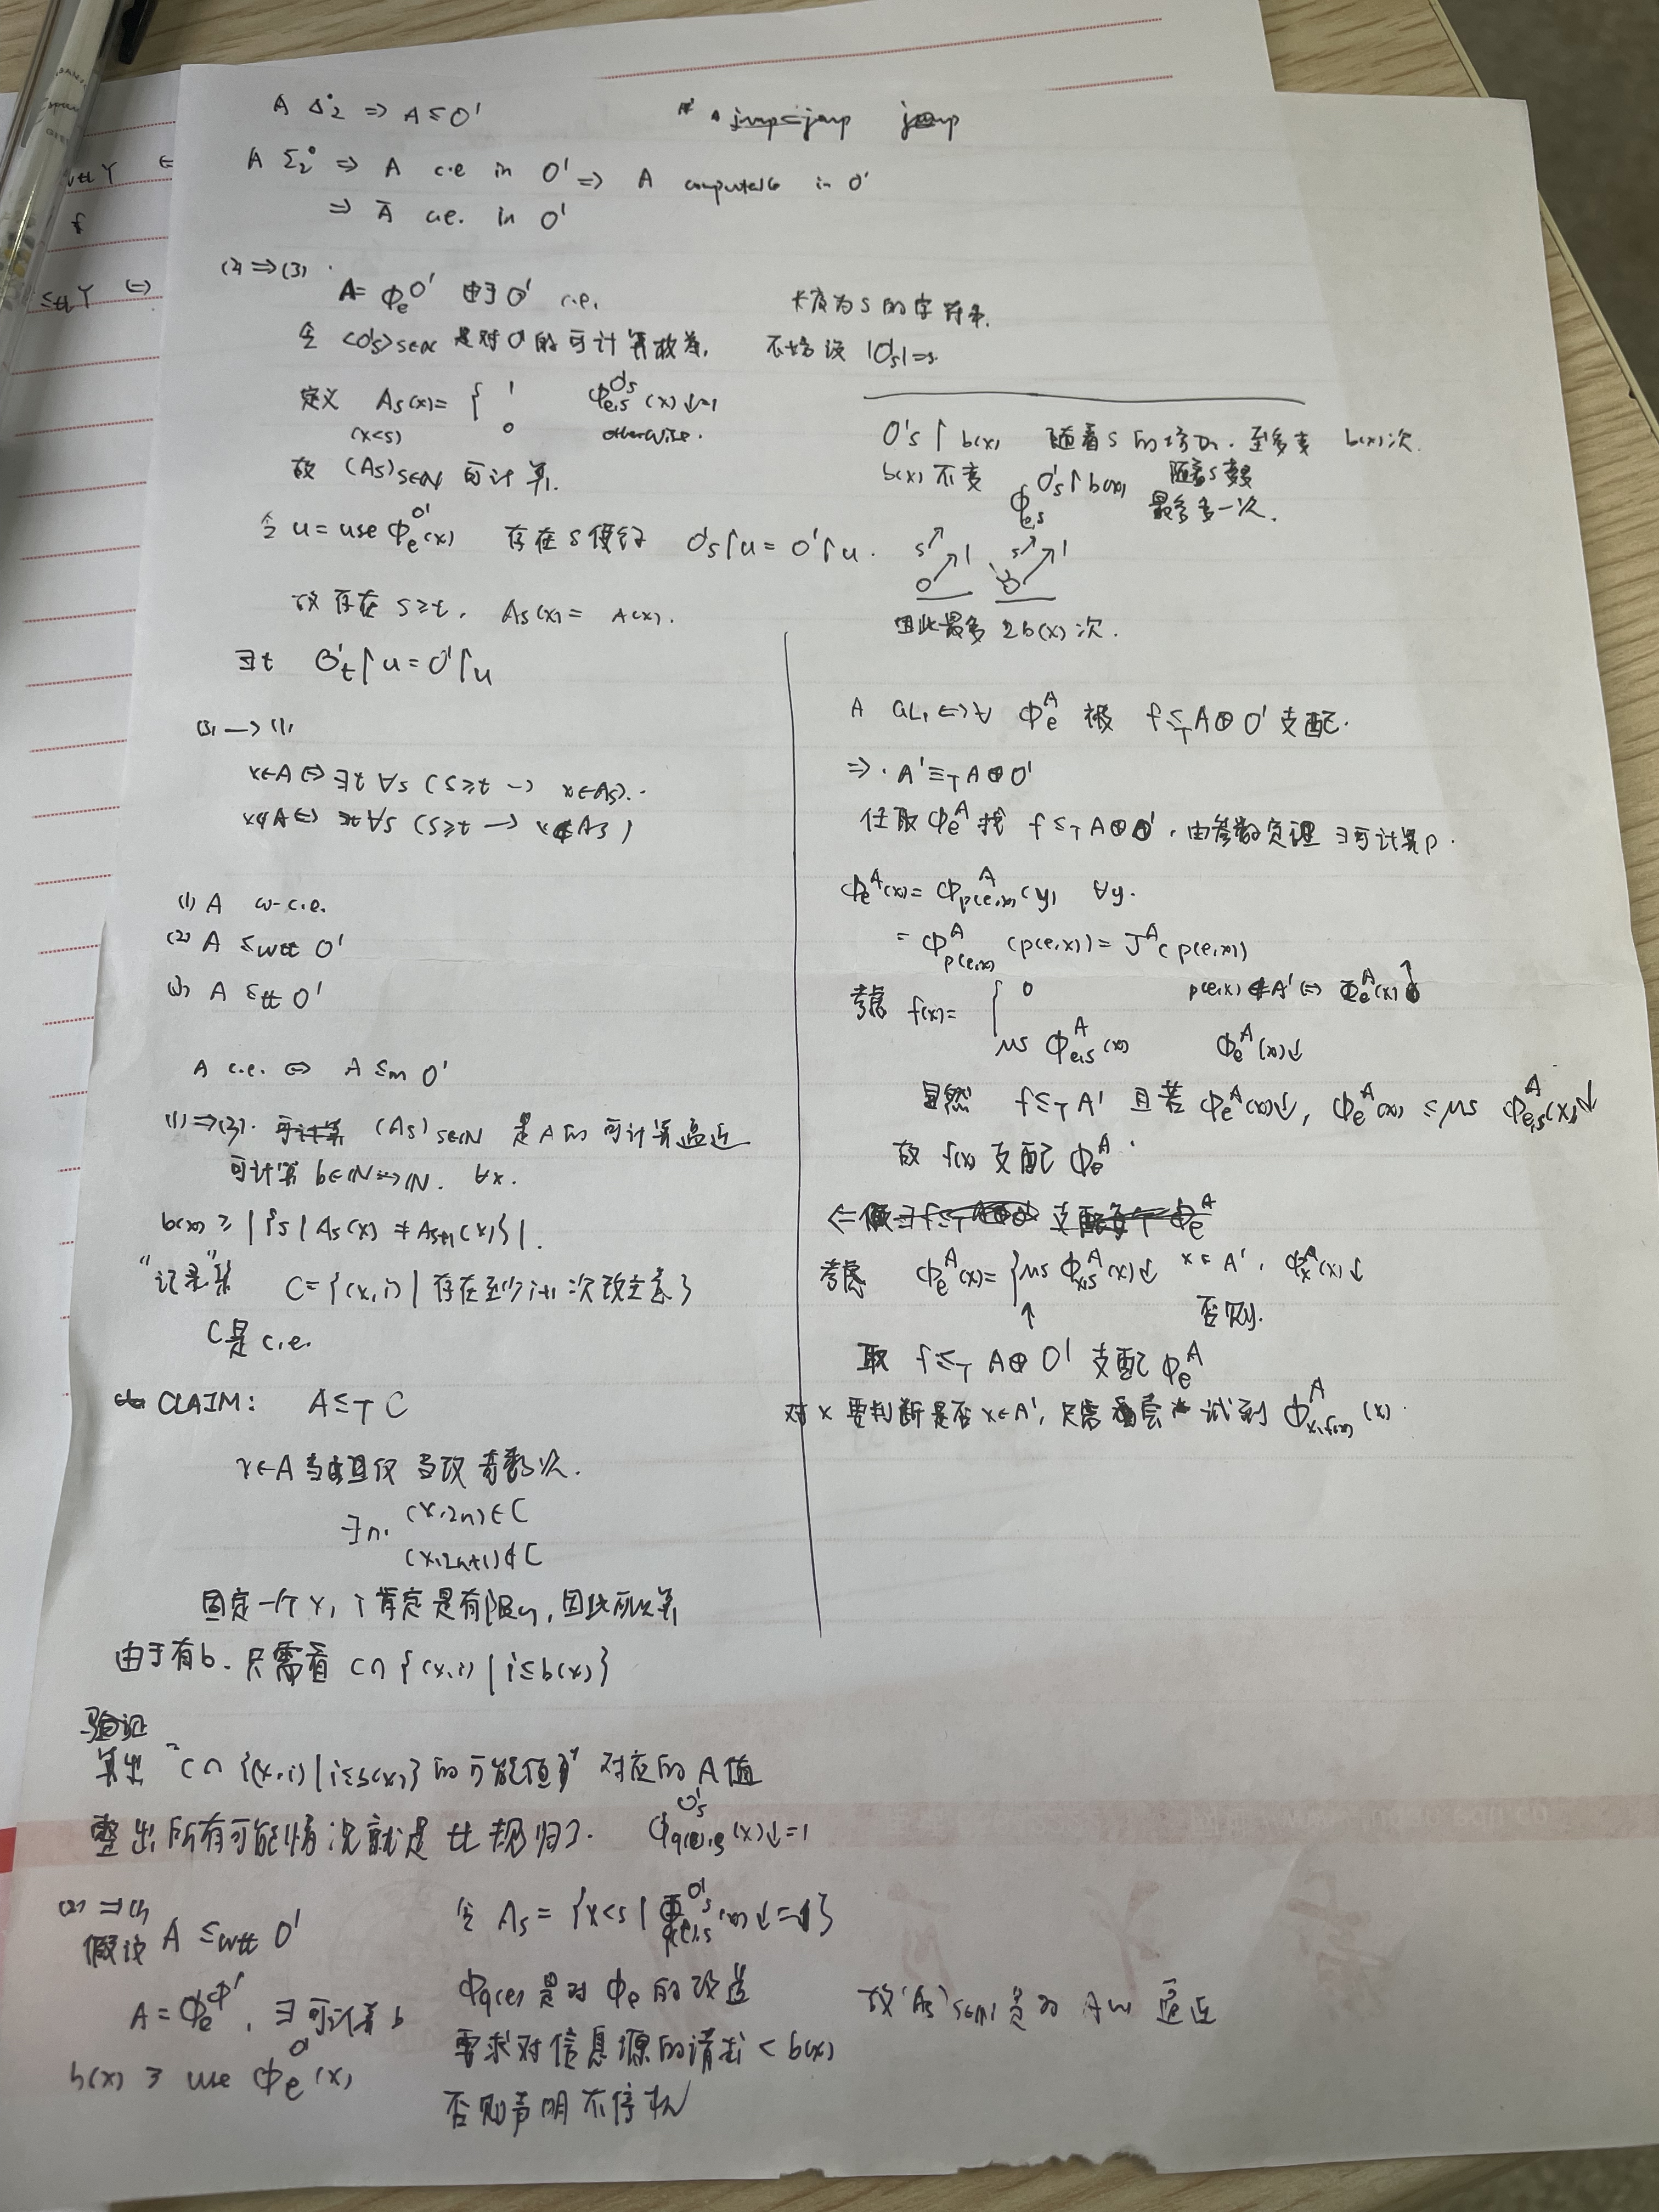
\includegraphics[width=\textwidth]{../images/6.824/1.png}
\label{}
\end{figure}

When the user program calls the \texttt{MapReduce} function, the following sequence of actions occurs
\begin{enumerate}
\item the MapReduce library in the user program first splits the input files into \(M\) pieces and
starts up many copies of the program on a cluster of machines
\item one of the copies of the program is special - the master. The rest are workers that are
assigned work by the master. there are \(M\) map tasks and \(R\) reduce tasks to assign. The
master picks idle workers and assigns each one a map task or a reduce task
\item 
\end{enumerate}
\end{document}
